\section{Poisson's Equation} 
Before detailing how to obtain an indicator function from the divergence of $\vec{V}(\vect{x})$, we discuss a general framework for solving Poisson's equation on a rectangular domain. We provide an analysis in $s$-dimensions, as this generalization comes at little cost. Explicitly, we seek an approximation of the function $\chi(\vect{x})$ that satisfies the Poisson equation with homogeneous Dirichlet boundary conditions, i.e. 
\begin{equation} \label{eq:PoissonEquation}
	\begin{split}
		\laplacian{\chi} &= f, \;\; \text{in} \;\; \oucube^s, \\
		\chi &= 0, \;\; \text{on} \;\; \partial \ucube^s,
	\end{split}
\end{equation}
where $\laplacian$ is the $s$-dimensional Laplace operator and
$\partial \ucube^s$ denotes the boundary of $\ucube^s$,
i.e. $\partial \ucube^s \cup \oucube^s = \ucube^s$.

\subsection{Greens Function}
The Poisson equation is an example of a well-studied partial differential equation. When the domain of interest is the unit cube $\ucube^s$, the solution can be analytically expressed in terms of a Green's function $\mathsf{G}(\vect{x},\vect{y})$ that represents the potential due to a point source placed at the location $\vect{x}$ inside $\ucube^s$.  In other words $\laplacian_{\vect{x}} \mathsf{G}(\vect{x},\vect{y}) = \delta(\vect{x}-\vect{y})$. The Green's function $\mathsf{G}$ has the Fourier Sine series expansion 
\begin{equation}
	\mathsf{G}(\vect{x},\vect{y}) = \sum_{\vect{m} \in \ints^s_+} 
	\frac{\prod_{i=1}^s \sin(m_i \pi x_i) \sin(m_i \pi y_i)}
	{-\pi^2 \norm{\vect{m}}^2},
	\label{eq:green}
\end{equation}
and the solution $\chi$ is given by
\begin{equation}
	\chi(\vect{x}) = \int_{\ucube^s}f(\vect{y})\mathsf{G}(\vect{x},\vect{y}) d\vect{y}.
	\label{eq:analytic}
\end{equation}


\subsection{Fourier Interpretation}

Even though there has been much effort on finding alternate rapidly
convergent series representations of the Green's function (see
e.g. Marshall~\cite{marshall99}), it turns out that the form of the
Green's function given in~\eqref{eq:green}, is ideally suited
for our needs as it allows us to easily express the solution in the
Fourier domain in terms of the Fourier coefficients of $f$.

Suppose we are given an $L_2(\ucube^s)$ function $\rho(
\vect{x})$ that is
defined on the open unit cube $\oucube^s$. In order to obtain a
Fourier sine series that converges to $\rho$ almost everywhere in
$\oucube^s$, we need to extend $\rho$ periodically such that it is odd
with respect to each variable. Particularly, let us extend the domain
of $\rho$ so that, within the interval $\cube^s$, it satisfies
{\small
\begin{equation}  
 \rho(\vect{x}) :=  
\begin{cases}
\bigl( \prod_{i=1}^s \sgn(x_i) \bigr)
\rho(|x_1|, \ldots, |x_s| ) &\mbox{if } \forall i \; |x_i| \ne 0 \\ 
0 &\mbox{otherwise},
\end{cases}
\label{eq:oddextension}
\end{equation}
}

while outside $\cube^s$, it is $\cube^s$-periodic, i.e. $\rho(\vect{x}
+ 2\vect{k}) = \rho(\vect{x})$ for $\vect{k} \in \ints^s$. The
extended function $\rho$ can be developed into a multidimensional
Fourier sine series, the coefficients of which are given by 
\begin{equation}
  \st{\rho}[\vect{m}] = 2^s \innerproduct{\rho(\vect{x})}
  {\textstyle{\prod_{i=1}^s}\sin(m_i\pi x_i)}, \; \text{for}\; \vect{m} \in \ints^s_+.
\end{equation}
The coefficient sequence $\st{\rho}[\vect{m}]$ can also be seen as a
special case of the more general multidimensional Fourier
series. In fact, with an odd extension of the sequence $\st{\rho}$, the
function $\rho$ can be expressed as a Fourier series. In particular,
if we define the Fourier series coefficients $\ft{\rho}[\vect{m}]$
(for $\vect{m} \in \ints^s$) as
{\small \begin{equation}
	\ft{\rho}[\vect{m}] := 
	\begin{cases}
	\frac{1}{(2\imath)^{s}} \prod_i \sgn(m_i)
	\st{\rho}[|m_1|,\ldots,|m_s|] &\mbox{if } \forall i \; |m_i| \ne 0 \\
	0 &\mbox{otherwise},
	\end{cases}
	\label{eq:oddFourierExtension}
\end{equation}}

then  $\rho$ is also given by the Fourier series
$
  \rho(\vect{x}) = \sum_{\vect{m} \in
    \ints^s} \ft{\rho}[\vect{m}] 
\exp(\imath \pi \vect{m} \cdot \vect{x})
$.
Thus, we use the notation $\st{\rho}[\cdot]$ and $\ft{\rho}[\cdot]$ to
distinguish between the Fourier sine series and Fourier series
coefficients of the periodic function $\rho$.
%Note that in the above equation, $\ft{\rho}[\vect{m}]$
%denotes the Fourier series of $\rho$ and is valid for all $\vect{m} \in
%\ints^s$.

Since the Green's function $\mathsf{G}$ is defined in $\oucube^s$ and has a
Fourier sine series representation, it is natural to seek a solution
that can be developed into a Fourier sine series as
well. Consequently, for the remainder of this section, we shall only
be dealing with Fourier sine series. Therefore, it suffices to
consider only the coefficients in $\ints^s_+$.

Using the analytic solution~\eqref{eq:analytic} and the sine series
representation of the Green's function~\eqref{eq:green}, it is easy to show that
the solution is given by
\begin{equation}
  \st{\chi}[\vect{m}] = -
  \frac{\st{f}[\vect{m}]}{\pi^2 \norm{\vect{m}}^2},
\label{eq:fourierSolution}
\end{equation}
where $\vect{m} \in \ints^s_+$ and $\st{f}[\cdot]$ represents the Fourier
sine series coefficients of the odd extension of $f$. To facilitate subsequent
discussions, let us introduce the solution operator
$\stpairs{\invlaplacian}{\frac{1}{-\pi^2 \norm{\vect{m}}^2}}$  ($\vect{m} \in
\ints^s_+$), where the symbol $\stpairs{}{}$ represents how the Fourier sine
series coefficients are affected by the operator.
%\begin{equation}
%V(\vect{x}) = \invlaplacian\Bigl( f(\vect{x}) +
%\sum_{i=1}^s D^0_i g^0_i(\vect{x}) + D^1_i g^1_i(\vect{x}) \bigr), 
%\label{eq:operatorAnalytic}
%\end{equation}
The self-adjoint operator $\invlaplacian$ is the inverse of the Laplace
operator. Self-adjointness can be easily verified with
the aid of Parseval's relation, which states that
$
  \innerproduct{a}{b} = \sum_{\vect{m} \in \ints^s_+} \st{a}[\vect{m}]
  \st{b}[\vect{m}] 
$
for any $\cube^s$-periodic functions $a$ and $b$ that are in
$L_2(\cube^s)$ and odd.



\subsection{Approximate Solution} \sec{sub:approximatesol}
We are interested in the scenario where the function $f$ is only known
through its point samples. Specifically, we assume that the samples of
$f$ reside on the sites of the lattice $\lattice{L}_h$. For the
purpose of enumerating the samples that are contained within
$\cube^s$, let us define the point set
\begin{equation}
  \pointset{T}_h := \underbrace{\{\vect{x}_1,\ldots,\vect{x}_{2^sN} \}}_{\pointset{I}_h}
  \cup
\underbrace{\{\vect{x}_{2^sN + 1},\ldots,\vect{x}_{2^sN + M} \}}_{\pointset{B}_h},
\end{equation}
where $\pointset{I}_h := \ocube^s \cap \{\vect{x} + \vect{m} :
\vect{x} \in \lattice{L}_h \cap \oucube^s, \vect{m} \in \ints^s \}$
consists of interior lattice points, while $\pointset{B}_h$ consists
of extended boundary points, i.e. $\pointset{B}_h := (\lattice{L}_h
\cap \partial\cube^s \cap (-1,1]^s) \cup (\lattice{L}_h \cap
\ocube^s\backslash \pointset{I}_h)$. Two dimensional illustrations are
shown in Figure~\ref{fig:pointset}. We note that with the above
definition of $\pointset{I}_h$, the points $\vect{x}_j$ for $j \in
\{1, \ldots, N\}$ are contained in the open unit cube $\oucube^s$
whereas the remaining points ($\vect{x}_j$ for $j \in \{N+1, \ldots,
2^sN\}$) lie outside. Furthermore, we assume
that the lattice $\lattice{L}$ and the sampling rate $h$ are such that
the set $\{\vect{x} + 2\vect{m} : \vect{x} \in \pointset{T}_h,
\vect{m} \in \ints^s\} = \lattice{L}_h$. We remark that this
requirement for $\lattice{L}_h$ is also
satisfied by integration lattices that are commonly used
to devise quadrature rules within the unit cube $\ucube^s$~\cite{nied92}.
\begin{figure}[t]
  \centering
  \subfloat[Cartesian]{\label{fig:cartesian}% This file is generated by the MATLAB m-file laprint.m. It can be included
% into LaTeX documents using the packages graphicx, color and psfrag.
% It is accompanied by a postscript file. A sample LaTeX file is:
%    \documentclass{article}\usepackage{graphicx,color,psfrag}
%    \begin{document}% This file is generated by the MATLAB m-file laprint.m. It can be included
% into LaTeX documents using the packages graphicx, color and psfrag.
% It is accompanied by a postscript file. A sample LaTeX file is:
%    \documentclass{article}\usepackage{graphicx,color,psfrag}
%    \begin{document}% This file is generated by the MATLAB m-file laprint.m. It can be included
% into LaTeX documents using the packages graphicx, color and psfrag.
% It is accompanied by a postscript file. A sample LaTeX file is:
%    \documentclass{article}\usepackage{graphicx,color,psfrag}
%    \begin{document}\input{2DCartesian}\end{document}
% See http://www.mathworks.de/matlabcentral/fileexchange/loadFile.do?objectId=4638
% for recent versions of laprint.m.
%
% created by:           LaPrint version 3.16 (13.9.2004)
% created on:           13-Dec-2011 13:39:05
% eps bounding box:     15 cm x 11.25 cm
% comment:              
%
\begin{psfrags}%
\psfragscanon%
%
% text strings:
\psfrag{s05}[lb][lb]{\color[rgb]{0,0,0}\setlength{\tabcolsep}{0pt}\begin{tabular}{l}$\;(1,1)$\end{tabular}}%
  \psfrag{s06}[rt][rt]{\color[rgb]{0,0,0}\setlength{\tabcolsep}{0pt}\begin{tabular}{r}$(-1,-1)$\end{tabular}}%
%
% xticklabels:
\psfrag{x01}[t][t]{-1}%
\psfrag{x02}[t][t]{-0.5}%
\psfrag{x03}[t][t]{0}%
\psfrag{x04}[t][t]{0.5}%
\psfrag{x05}[t][t]{1}%
%
% yticklabels:
\psfrag{v01}[r][r]{-1}%
\psfrag{v02}[r][r]{-0.8}%
\psfrag{v03}[r][r]{-0.6}%
\psfrag{v04}[r][r]{-0.4}%
\psfrag{v05}[r][r]{-0.2}%
\psfrag{v06}[r][r]{0}%
\psfrag{v07}[r][r]{0.2}%
\psfrag{v08}[r][r]{0.4}%
\psfrag{v09}[r][r]{0.6}%
\psfrag{v10}[r][r]{0.8}%
\psfrag{v11}[r][r]{1}%
%
% Figure:
\resizebox{0.4\columnwidth}{!}{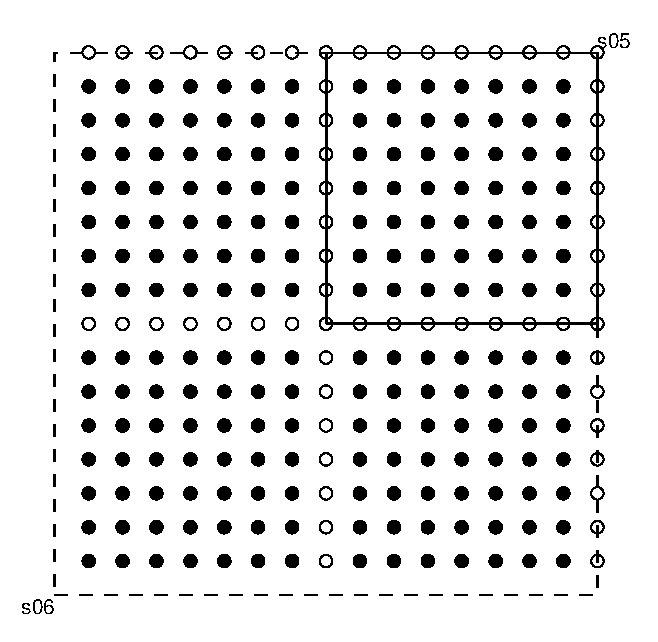
\includegraphics{./figures/2DCartesian.eps}}%
\end{psfrags}%
%
% End 2DCartesian.tex
\end{document}
% See http://www.mathworks.de/matlabcentral/fileexchange/loadFile.do?objectId=4638
% for recent versions of laprint.m.
%
% created by:           LaPrint version 3.16 (13.9.2004)
% created on:           13-Dec-2011 13:39:05
% eps bounding box:     15 cm x 11.25 cm
% comment:              
%
\begin{psfrags}%
\psfragscanon%
%
% text strings:
\psfrag{s05}[lb][lb]{\color[rgb]{0,0,0}\setlength{\tabcolsep}{0pt}\begin{tabular}{l}$\;(1,1)$\end{tabular}}%
  \psfrag{s06}[rt][rt]{\color[rgb]{0,0,0}\setlength{\tabcolsep}{0pt}\begin{tabular}{r}$(-1,-1)$\end{tabular}}%
%
% xticklabels:
\psfrag{x01}[t][t]{-1}%
\psfrag{x02}[t][t]{-0.5}%
\psfrag{x03}[t][t]{0}%
\psfrag{x04}[t][t]{0.5}%
\psfrag{x05}[t][t]{1}%
%
% yticklabels:
\psfrag{v01}[r][r]{-1}%
\psfrag{v02}[r][r]{-0.8}%
\psfrag{v03}[r][r]{-0.6}%
\psfrag{v04}[r][r]{-0.4}%
\psfrag{v05}[r][r]{-0.2}%
\psfrag{v06}[r][r]{0}%
\psfrag{v07}[r][r]{0.2}%
\psfrag{v08}[r][r]{0.4}%
\psfrag{v09}[r][r]{0.6}%
\psfrag{v10}[r][r]{0.8}%
\psfrag{v11}[r][r]{1}%
%
% Figure:
\resizebox{0.4\columnwidth}{!}{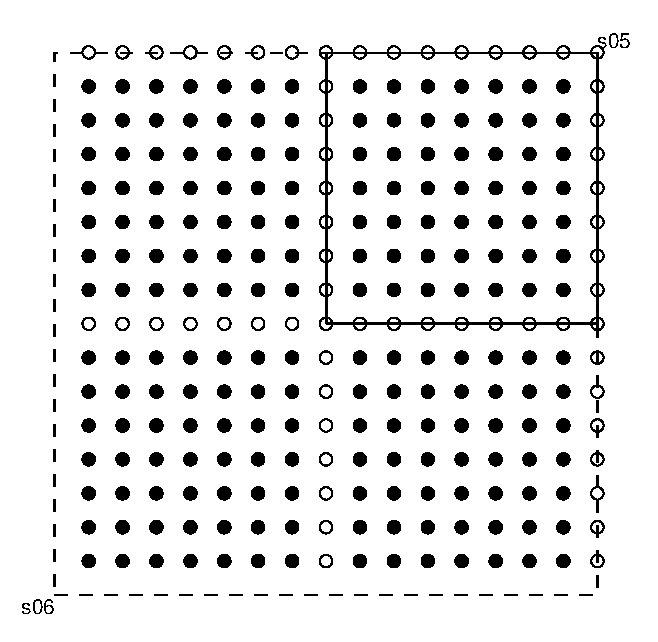
\includegraphics{./figures/2DCartesian.eps}}%
\end{psfrags}%
%
% End 2DCartesian.tex
\end{document}
% See http://www.mathworks.de/matlabcentral/fileexchange/loadFile.do?objectId=4638
% for recent versions of laprint.m.
%
% created by:           LaPrint version 3.16 (13.9.2004)
% created on:           13-Dec-2011 13:39:05
% eps bounding box:     15 cm x 11.25 cm
% comment:              
%
\begin{psfrags}%
\psfragscanon%
%
% text strings:
\psfrag{s05}[lb][lb]{\color[rgb]{0,0,0}\setlength{\tabcolsep}{0pt}\begin{tabular}{l}$\;(1,1)$\end{tabular}}%
  \psfrag{s06}[rt][rt]{\color[rgb]{0,0,0}\setlength{\tabcolsep}{0pt}\begin{tabular}{r}$(-1,-1)$\end{tabular}}%
%
% xticklabels:
\psfrag{x01}[t][t]{-1}%
\psfrag{x02}[t][t]{-0.5}%
\psfrag{x03}[t][t]{0}%
\psfrag{x04}[t][t]{0.5}%
\psfrag{x05}[t][t]{1}%
%
% yticklabels:
\psfrag{v01}[r][r]{-1}%
\psfrag{v02}[r][r]{-0.8}%
\psfrag{v03}[r][r]{-0.6}%
\psfrag{v04}[r][r]{-0.4}%
\psfrag{v05}[r][r]{-0.2}%
\psfrag{v06}[r][r]{0}%
\psfrag{v07}[r][r]{0.2}%
\psfrag{v08}[r][r]{0.4}%
\psfrag{v09}[r][r]{0.6}%
\psfrag{v10}[r][r]{0.8}%
\psfrag{v11}[r][r]{1}%
%
% Figure:
\resizebox{0.4\columnwidth}{!}{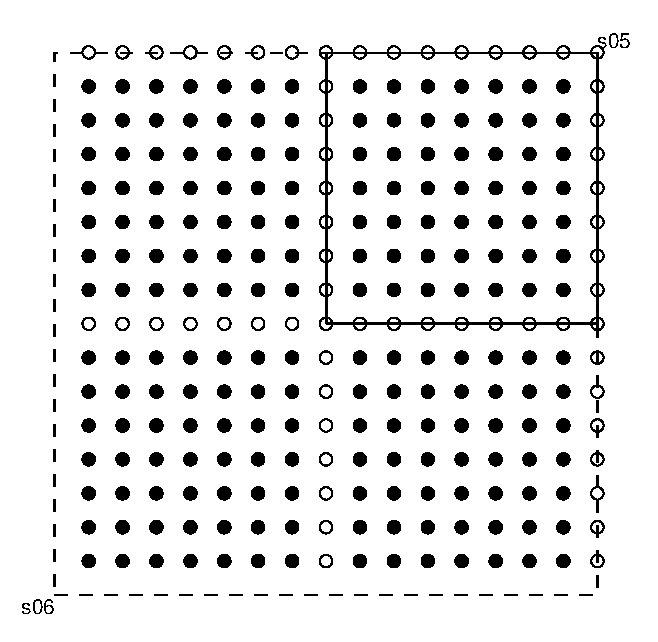
\includegraphics{./figures/2DCartesian.eps}}%
\end{psfrags}%
%
% End 2DCartesian.tex
}
  \hspace{2em}
  \subfloat[Quincunx]{\label{fig:quincunx}% This file is generated by the MATLAB m-file laprint.m. It can be included
% into LaTeX documents using the packages graphicx, color and psfrag.
% It is accompanied by a postscript file. A sample LaTeX file is:
%    \documentclass{article}\usepackage{graphicx,color,psfrag}
%    \begin{document}% This file is generated by the MATLAB m-file laprint.m. It can be included
% into LaTeX documents using the packages graphicx, color and psfrag.
% It is accompanied by a postscript file. A sample LaTeX file is:
%    \documentclass{article}\usepackage{graphicx,color,psfrag}
%    \begin{document}% This file is generated by the MATLAB m-file laprint.m. It can be included
% into LaTeX documents using the packages graphicx, color and psfrag.
% It is accompanied by a postscript file. A sample LaTeX file is:
%    \documentclass{article}\usepackage{graphicx,color,psfrag}
%    \begin{document}\input{2DQuincunx}\end{document}
% See http://www.mathworks.de/matlabcentral/fileexchange/loadFile.do?objectId=4638
% for recent versions of laprint.m.
%
% created by:           LaPrint version 3.16 (13.9.2004)
% created on:           13-Dec-2011 13:39:19
% eps bounding box:     15 cm x 11.25 cm
% comment:              
%
\begin{psfrags}%
\psfragscanon%
%
% text strings:
\psfrag{s05}[lb][lb]{\color[rgb]{0,0,0}\setlength{\tabcolsep}{0pt}\begin{tabular}{l}$\;(1,1)$\end{tabular}}%
\psfrag{s06}[rt][rt]{\color[rgb]{0,0,0}\setlength{\tabcolsep}{0pt}\begin{tabular}{r}$(-1,-1)$\end{tabular}}%
%
% xticklabels:
\psfrag{x01}[t][t]{-1}%
\psfrag{x02}[t][t]{-0.5}%
\psfrag{x03}[t][t]{0}%
\psfrag{x04}[t][t]{0.5}%
\psfrag{x05}[t][t]{1}%
%
% yticklabels:
\psfrag{v01}[r][r]{-1}%
\psfrag{v02}[r][r]{-0.8}%
\psfrag{v03}[r][r]{-0.6}%
\psfrag{v04}[r][r]{-0.4}%
\psfrag{v05}[r][r]{-0.2}%
\psfrag{v06}[r][r]{0}%
\psfrag{v07}[r][r]{0.2}%
\psfrag{v08}[r][r]{0.4}%
\psfrag{v09}[r][r]{0.6}%
\psfrag{v10}[r][r]{0.8}%
\psfrag{v11}[r][r]{1}%
%
% Figure:
\resizebox{0.4\columnwidth}{!}{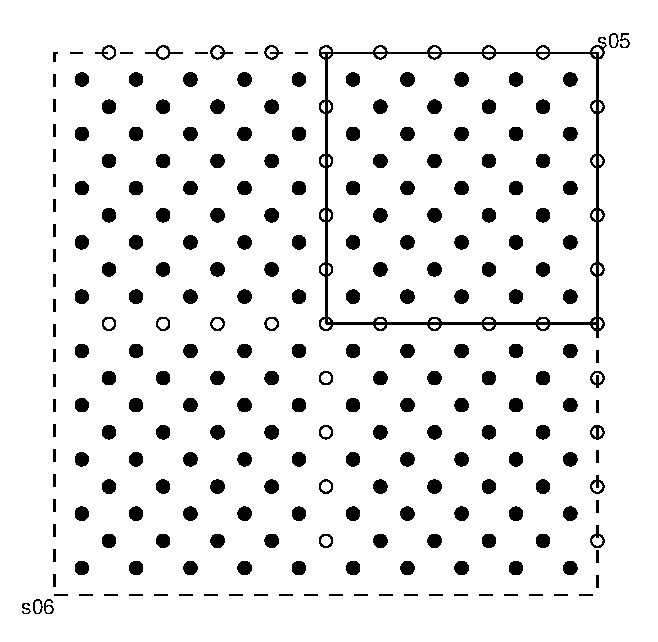
\includegraphics{./figures/2DQuincunx.eps}}%
\end{psfrags}%
%
% End 2DQuincunx.tex
\end{document}
% See http://www.mathworks.de/matlabcentral/fileexchange/loadFile.do?objectId=4638
% for recent versions of laprint.m.
%
% created by:           LaPrint version 3.16 (13.9.2004)
% created on:           13-Dec-2011 13:39:19
% eps bounding box:     15 cm x 11.25 cm
% comment:              
%
\begin{psfrags}%
\psfragscanon%
%
% text strings:
\psfrag{s05}[lb][lb]{\color[rgb]{0,0,0}\setlength{\tabcolsep}{0pt}\begin{tabular}{l}$\;(1,1)$\end{tabular}}%
\psfrag{s06}[rt][rt]{\color[rgb]{0,0,0}\setlength{\tabcolsep}{0pt}\begin{tabular}{r}$(-1,-1)$\end{tabular}}%
%
% xticklabels:
\psfrag{x01}[t][t]{-1}%
\psfrag{x02}[t][t]{-0.5}%
\psfrag{x03}[t][t]{0}%
\psfrag{x04}[t][t]{0.5}%
\psfrag{x05}[t][t]{1}%
%
% yticklabels:
\psfrag{v01}[r][r]{-1}%
\psfrag{v02}[r][r]{-0.8}%
\psfrag{v03}[r][r]{-0.6}%
\psfrag{v04}[r][r]{-0.4}%
\psfrag{v05}[r][r]{-0.2}%
\psfrag{v06}[r][r]{0}%
\psfrag{v07}[r][r]{0.2}%
\psfrag{v08}[r][r]{0.4}%
\psfrag{v09}[r][r]{0.6}%
\psfrag{v10}[r][r]{0.8}%
\psfrag{v11}[r][r]{1}%
%
% Figure:
\resizebox{0.4\columnwidth}{!}{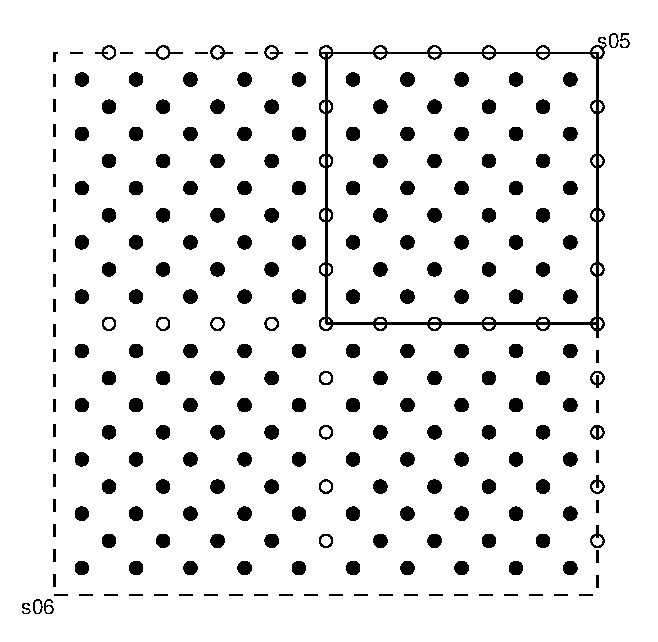
\includegraphics{./figures/2DQuincunx.eps}}%
\end{psfrags}%
%
% End 2DQuincunx.tex
\end{document}
% See http://www.mathworks.de/matlabcentral/fileexchange/loadFile.do?objectId=4638
% for recent versions of laprint.m.
%
% created by:           LaPrint version 3.16 (13.9.2004)
% created on:           13-Dec-2011 13:39:19
% eps bounding box:     15 cm x 11.25 cm
% comment:              
%
\begin{psfrags}%
\psfragscanon%
%
% text strings:
\psfrag{s05}[lb][lb]{\color[rgb]{0,0,0}\setlength{\tabcolsep}{0pt}\begin{tabular}{l}$\;(1,1)$\end{tabular}}%
\psfrag{s06}[rt][rt]{\color[rgb]{0,0,0}\setlength{\tabcolsep}{0pt}\begin{tabular}{r}$(-1,-1)$\end{tabular}}%
%
% xticklabels:
\psfrag{x01}[t][t]{-1}%
\psfrag{x02}[t][t]{-0.5}%
\psfrag{x03}[t][t]{0}%
\psfrag{x04}[t][t]{0.5}%
\psfrag{x05}[t][t]{1}%
%
% yticklabels:
\psfrag{v01}[r][r]{-1}%
\psfrag{v02}[r][r]{-0.8}%
\psfrag{v03}[r][r]{-0.6}%
\psfrag{v04}[r][r]{-0.4}%
\psfrag{v05}[r][r]{-0.2}%
\psfrag{v06}[r][r]{0}%
\psfrag{v07}[r][r]{0.2}%
\psfrag{v08}[r][r]{0.4}%
\psfrag{v09}[r][r]{0.6}%
\psfrag{v10}[r][r]{0.8}%
\psfrag{v11}[r][r]{1}%
%
% Figure:
\resizebox{0.4\columnwidth}{!}{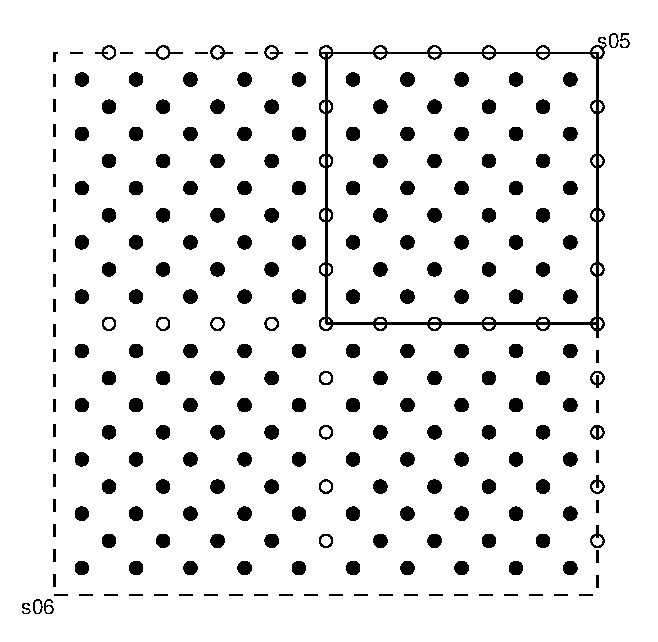
\includegraphics{./figures/2DQuincunx.eps}}%
\end{psfrags}%
%
% End 2DQuincunx.tex
}
  \caption[Interior and boundary samples]{Illustration of the point set
  $\pointset{T}_h$ on the two
    dimensional Cartesian ($\mat{L} = \bigl( \begin{smallmatrix} 1&0\\
      0&1
    \end{smallmatrix} \bigr)$, $h=\tfrac{1}{8}$) and Quincunx ($\mat{L} = \bigl(
    \begin{smallmatrix} 1&-1\\
      1&1
    \end{smallmatrix} \bigr)$, $h=\tfrac{1}{10}$) lattices. The interior points
    ($\bullet$) belong to the set $\pointset{I}_h$ while the extended
    boundary points ($\circ$) belong to $\pointset{B}_h$.}
  \label{fig:pointset}
\end{figure}

We denote the interior samples of $f$ as $f[\vect{x}_j] :=
f(\vect{x}_j)$ where $\vect{x}_j \in \pointset{I}_h$. Note that
$f[\vect{x}_j]$ only needs to be known in $\oucube^s$ ($j \in
\{1,\ldots,N\}$), the other samples can be inferred from
oddity. 

We wish to use the samples of $f$ to approximate the function $\chi$ that solves the Poisson equation~\eqref{eq:PoissonEquation}. Since
$\chi$ is a periodic function, we follow the recipe of Jacob \textit{et al.}~\cite{jacob02} and seek an approximation that lies in a space generated by a periodic reconstruction function. Specifically, we are interested in the case
where $\appf{\chi}$ lies in the space $\aspace{\lattice{L}_h}{\varphi_p} := \mathrm{span}_{\vect{x}_j\in\pointset{T}_h}\{
\varphi_p(\frac{\vect{x}-\vect{x}_j}{h}) \}$ that is spanned by the scaled and translated versions of a periodic function $\varphi_p$. Our approximation is given by
\begin{equation}
  \appf{\chi}(\vect{x}) = \sum_{\vect{x}_j \in \pointset{T}_h} c[\vect{x}_j] 
\varphi_p\bigl(\frac{\vect{x} - \vect{x}_j}{h}\bigr),
\label{eq:ansatz}
\end{equation}
where $c[\vect{x}_j]$ is an unknown coefficient sequence defined on the point set $\pointset{T}_h$ that is to be determined from the samples of $f$. The function $\varphi_p$ is a periodized version of a generating function $\varphi$ and is defined as
\begin{equation}
\varphi_p(\vect{x}) := \sum_{\vect{m} \in \ints^s} 
\varphi\bigl(\vect{x} - \frac{2}{h} \vect{m} \bigr).
\label{eq:periodization}
\end{equation}

%\begin{figure}[t]
 % \centering
 % \subfloat[$\cbs^3(x)$]{\includegraphics[width=0.28\columnwidth]
  %{./figures/periodization/cubic}}
  %\hspace{2em}
  %\subfloat[$\cbs^3_p(x)$]{\includegraphics[width=0.28\columnwidth]
  %{./figures/periodization/cubicPeriodized}}
  %\hspace{2em}
  %\subfloat[$\cbs^3_p(\tfrac{x}{h})$]{\includegraphics[width=0.28\columnwidth]
  %{./figures/periodization/cubicPeriodizedScaled}}
  %\caption[Making a generator periodic]{1D illustration of the periodization
  %operation defined by~\eqref{eq:periodization}: $\varphi(x) = \cbs^3(x)$
  %and $h = 0.2$.}
  %\label{fig:periodization}
%\end{figure}

It is easy to verify that, with this definition of $\varphi_p$,
$\appf{\chi}$ is also $\cube^s$-periodic. Even though we are only
interested in the behavior of $\appf{V}$ inside $\ucube^s$, extending $\appf{\chi}$ to the entire domain $\cube^s$ using~\eqref{eq:ansatz} allows us to use the Fourier domain error kernel proposed by Jacob \textit{et. al}~\cite{jacob02} to quantify the approximation error $\LLnorm{\chi - \appf{\chi}}$.

Another simplification is in order here. Since the solution $\chi$ to the Poisson problem~\eqref{eq:PoissonEquation} is odd with respect to each variable, we look for an approximate solution $\appf{\chi} \in \aspace{\lattice{L}_h}{\varphi_p}$
that is also odd in each variable. This can be achieved by setting
the boundary coefficients to zero and by requiring that the resulting sequence be odd.  With $c[\vect{x}_j] = 0$ for $\vect{x}_j \in \pointset{B}_h$, the approximation~\eqref{eq:ansatz} simplifies to
\begin{equation}
\appf{V}(\vect{x}) = \sum_{j=1}^{2^sN} c[\vect{x}_j] 
\varphi_p(\frac{\vect{x} - \vect{x}_j}{h}).
\label{eq:simplifiedAnsatz}
\end{equation}
If the generator $\varphi$ is even and the sequence $c[\cdot]$ is odd,
the resulting approximation $\appf{V}$ is odd and satifies zero
Dirichlet boundary conditions (see Appendix~\ref{app:1}). With this
simplification, the coefficient sequence $c[\vect{x}_j]$ only needs to
be determined for $j \in \{1,\ldots,N\}$. The rest can be inferred
from oddity.  

\subsection{Error Analysis}

\subsubsection{Error Kernel for Periodic Functions}
\label{sec:periodicErrorKernel}
In many approximation problems involving periodic functions, one is interested
in seeking an approximation $\appf{z}$ of a periodic function $z$ from its
measurements that lie on some sampling lattice. In light of the notations
introduced earlier, suppose that $z \in L_2(\cube^s)$ and is also
$\cube^s$-periodic. Additionally, suppose that the measurements are made at the
locations $\vect{x}_j \in \pointset{T}_h$ so that one can obtain an
approximation $\appf{z}$ that belongs to  $\aspace{\lattice{L}_h}{\varphi_p}$
and --- in a manner similar to the expansion~\eqref{eq:ansatz} --- is given by
$
  \appf{z}(\vect{x}) = \sum_{\vect{x}_j \in \pointset{T}_h}
  \zeta[\vect{x}_j] \varphi_p(\frac{\vect{x}-\vect{x}_j}{h}),
$
where the
coefficient sequence $\zeta[\cdot]$ is obtained through the discrete
measurements
\begin{equation}
  \zeta[\vect{x}_j] = \innerproduct{z(\vect{x})}{\analysis{\varphi}_p(\frac{\vect{x} - \vect{x}_j}{h})}
\label{eq:measurements}
\end{equation}
made with the scaled and shifted versions of a periodic analysis
function $\analysis{\varphi}_p(\vect{x})$ (the periodization operation
is defined by~\eqref{eq:periodization}). The main result of Jacob
\textit{et al.}~\cite{jacob02} states that the mean square
approximation error $\LLnorm{z - \appf{z}}$ at scale $h$ can
be predicted according to
\begin{equation}
  \sqrt{\sum_{\vect{m} \in \ints^s} \norm{\ft{z}[\vect{m}]}^2 E(\frac{h}{2}\vect{m})}
\label{eq:prediction}
\end{equation}
where $\ft{z}[\vect{m}]$ are the Fourier series coefficients of $z$
and $E(\cdot)$ is the error kernel of Blu and Unser~\cite{blu99}
introduced earlier~\eqref{eq:scErrorKernel}.  Remarkably, the same
error kernel can be used to predict the error for periodic and
non-periodic functions alike. The only change that needs to be made is
in the prediction equation. For functions in $L_2(\reel^s)$, the error
is predicted according to the integral in~\eqref{eq:avgError}. On the
other hand, for periodic functions that belong to $L_2(\cube^s)$, the
prediction equation turns into the summation given
in~\eqref{eq:prediction}. We refer the reader to Jacob \textit{et
  al.}~\cite{jacob02} for details.


\subsubsection{Extension to Linear Operators}
We are interested in approximating from the discrete measurements
of $z$, not the function $z$ itself but a function $\Gamma z$ that is obtained
by applying the linear operator $\Gamma$ to $z$. 
% This is exactly the problem we
% are faced with in the case of approximating the analytic
% solution~\eqref{eq:fourierSolution} to Poisson's equation. 
We would like to
extend the error kernel formulation~\eqref{eq:scErrorKernel} so that it will
allow us to quantify the error incurred in approximating $\Gamma z$ from the
measurements of $z$. Towards this end, we assume that the approximation
$\appf{(\Gamma z)}$ lies in a shift-invariant space spanned by the generator
$\varphi_p$, where the coefficients are obtained from the measurements through a
digital filtering operation. Particularly, we seek an approximation that is
given by
\begin{equation}
\appf{(\Gamma z)}(\vect{x}) = C_h \sum_{\vect{x}_j \in \pointset{T}_h} 
(\zeta \pconv \gamma_h)[\vect{x}_j]
\varphi_p(\frac{\vect{x}-\vect{x}_j}{h}),
\label{eq:opApproximation}
\end{equation}
where $\zeta$ denotes the discrete measurements of $z$ obtained
through~\eqref{eq:measurements}, $\gamma$ is a digital filter defined on
the lattice $\lattice{L}$ and $\gamma_h$ is its corresponding scaled
version, i.e. $\gamma_h[\vect{x}_j] := \gamma[\tfrac{\vect{x}_j}{h}]$ where
$\tfrac{\vect{x}_j}{h} \in \lattice{L}$, and $C_h$ is an associated
scaling constant. The digital filter $\gamma$ represents a suitable
discretization of the operator $\Gamma$ on the lattice $\lattice{L}$. It is
to be applied to the measurements through a cyclic convolution
operation (denoted by $\pconv$) on the lattice $\lattice{L}_h$ using a
periodized version of $\gamma_h$. In particular, the convolution operation
in~\eqref{eq:opApproximation} is defined as
\begin{equation}
  (\zeta \pconv \gamma_h)[\vect{x}_j] :=
  \sum_{\vect{x}_k \in \pointset{T}_h}
  \bigl(
    \sum_{\vect{m} \in \ints^s}\gamma[\frac{\vect{x}_k + 2\vect{m}}{h}]
  \bigr)
  \zeta[\vect{x}_j - \vect{x}_k],
\label{eq:cyclicConvolution}
\end{equation}
where $\vect{x}_j \in \lattice{L}_h$. In the above definition,
$\zeta[\cdot]$ is assumed to be $\cube^s$-periodic.  Furthermore, the
resulting sequence $(\zeta \pconv \gamma_h)[\cdot]$ is also
$\cube^s$-periodic.

% periodic boundary conditions on $\zeta$. Note that, even though $t$ is not
% periodic, the resulting convolution $\zeta \pconv t_h$ is since $\zeta$ itself
% is periodic.
Let $\ft{\Gamma}(\vect{\omega})$ be the Fourier transform of the operator
$\Gamma$, and $\ft{G}(\vect{\omega})$ be the DTFT of the filter $\gamma$.
Furthermore, let $\Gamma$ be bounded so that $\Gamma z \in L_2(\cube^s)$.
A simple modification of the measurement process~\eqref{eq:measurements} yields
the desired extension of the error kernel formulation~\eqref{eq:scErrorKernel}.
Our main result can be summarised as follows.
\begin{thm}
  Suppose that $\Gamma$ is self-adjoint and shift-invariant. The Fourier
  error kernel that predicts the approximation error
  $\LLnorm{\appf{(\Gamma z)} - \Gamma z}$ is given by $E(\vect{\omega}) :=
  E_{\mathsf{min}}(\vect{\omega}) + E_{\mathsf{mod}}(\vect{\omega})$,
  where the minimum error kernel $E_{\mathsf{min}}(\vect{\omega})$ is
  given in~\eqref{eq:scErrorKernel}, while the modified residue
  error kernel is given by
  \begin{equation}
    E_{\mathsf{mod}}(\vect{\omega}) = 
    \ft{A}_{\varphi}(\vect{\omega})
    \abs{
      \frac{\ft{\analysis{\varphi}}(\vect{\omega}) \ft{G}(\vect{\omega})}
      {\ft{\Gamma}(\vect{\omega})}
      - 
      \ft{\dual{\varphi}}(\vect{\omega})}^2.
    \label{eq:opResidue}
  \end{equation}
\label{thm:1}
\end{thm}
The proof is given in Appendix~\ref{app:proofs}.

Note that, even though the operator $\Gamma$ acts in the space $L_2(\cube^s)$,
it is extended to the more general space $L_2(\reel^s)$ in this error kernel
formulation.
Therefore,~\eqref{eq:opResidue} can be used to quantify the $L_2$ error in both
$L_2(\reel^s)$ and $L_2(\cube^s)$. Going back to the original
problem~\eqref{eq:PoissonEquation}, Theorem~\ref{thm:1} gives us a way to design
and analyze digital filtering solutions that approximate the analytic
solution~\eqref{eq:fourierSolution}. In particular, the linear operator that we
wish to discretize is $\invlaplacian$. In the sequel, we show how to use the
modified residue error kernel~\eqref{eq:opResidue} to design filtering schemes
that discretize this operator and can be efficiently implemented in the
Fourier domain.

In order to characterize the order of accuracy provided by a periodic
generating function $\varphi_p$, we shall switch to the more general
space $L_2(\reel^s)$.  The link between the approximation properties
of $\varphi$ and those of its periodized version $\varphi_p$ is
established by the error kernel formulation introduced
in~\SC{sec:periodicErrorKernel}. Since the same kernel can be used in
both cases, henceforth, we shall reason about the approximation
properties of the generator $\varphi$ as the same properties are also
applicable to its periodized counterpart $\varphi_p$.

In many approximation scenarios, one typically assumes a Dirac point sampling
model, i.e. $\analysis{\varphi}(\vect{x}) = \delta(\vect{x})$.
This prevents the direct realization of the minimum approximation scenario.
Furthermore, for many functions encountered in practice, the power spectrum is
concentrated around $\vect{\omega} = 0$. For such scenarios, one speaks of an
\emph{asymptotically optimal} $k$-th order approximation scheme if the $L_2$
error behaves as $O(h^k)$ where $k = \order{\lattice{L}}{\varphi}$. Our operator
discretization approach is also based on these assumptions. Provided that $\chi$ has appropriate smoothness, our goal is to design suitable digital filters that yield %$V \in W_2^k(\cube^s)$, our goal is to design suitable digital filters that yield
$\appf{\chi}$ such that $\LLnorm{\chi - \appf{chi}} = O(h^k)$. %As discussed earlier in~\SC{sec:interpQuasiInterp}, the criterion that needs to be satisfied is $E_{\mathsf{mod}}(\vect{\omega}) = O(\norm{\vect{\omega}}^{2k})$.

\subsection{Relationship to the Galerkin method}
\label{sec:Galerkin}
The modified residue error kernel~\eqref{eq:opResidue} can also be analyzed in light of the Galerkin method~\cite{quarteroni08} using a weak formulation of the Poisson equation~\eqref{eq:PoissonEquation}, where the trial and test spaces are the same with the notable difference that the spaces are not required to explicitly satisfy any particular boundary conditions. Rather, a zero boundary condition is implicitly obtained by requiring that the solution coefficients $c[\cdot]$ be odd as explained in~\SC{sub:approximatesol}. Here, we establish the connection for the homogeneous case but the analysis also easily extends to the non-homogeneous case, as well as to other types of differential operators.

In its weak form, the solution $\chi \in L_2(\cube^s)$ to the homogeneous Poisson equation~\eqref{eq:PoissonEquation} satisfies the weak formulation
\begin{equation}
  \innerproduct{\chi}{u} = \mathcal{F}(u), \;\; \forall u \in L_2(\cube^s),
\end{equation}
where the functions $u$ are suitable test functions. The functional
$\mathcal{F}(\cdot)$ is defined as $\mathcal{F}(u) :=
\innerproduct{\invlaplacian f}{u}$, where $f$ is the odd extension of
the function that appears on the right hand side
of~\eqref{eq:PoissonEquation}, and the operator
$\stpairs{\invlaplacian}{\tfrac{1}{-\pi^2\norm{\vect{m}}^2}}$ has the
interpretation of the inverse Laplacian as introduced
in~\eqref{eq:fourierSolution}. We remark that this formulation is
slightly stronger than the usual weak formulations based on the
Laplacian $\laplacian$ where the trial and test spaces coincide with
the Sobolev space $W_2^1(\cube^s)$. In comparison, here the trial and
test spaces coincide with the more general space $L_2(\cube^s)$. This
formulation is also in direct correspondence with our earlier
treatment of the problem.

Let us now restrict attention to the finite dimensional space
$\aspace{\lattice{L}_h}{\varphi_p} \subset L_2(\cube^s)$. We seek a
weak solution $\appf{\chi} \in \aspace{\lattice{L}_h}{\varphi_p}$ so that
\begin{equation}
  \innerproduct{\appf{\chi}}{u_h} = \mathcal{F}(u_h), \;\;
  \forall u_h \in \aspace{\lattice{L}_h}{\varphi_p},
\end{equation}
and the Galerkin residual satifies the orthogonality condition
\begin{equation}
  \innerproduct{\chi - \appf{\chi}}{u_h} = 0, \;\;
  \forall u_h \in \aspace{\lattice{L}_h}{\varphi_p}.
  \label{eq:GalerkinOrthogonality}
\end{equation}
From this, it can be deduced that the minimum error approximation $\appf{\chi}$ is the orthogonal projection of $\chi$ upon $\aspace{\lattice{L}_h}{\varphi_p}$. The coefficients of the approximation are thus given by
\begin{equation}
  \begin{split}
    c[\vect{x}_j] & = \mathcal{F}(h^{-s}
    \dual{\varphi}(\frac{\vect{x}-\vect{x}_j}{h})) \\
    & = 
    \innerproduct{f(\vect{x})}{\invlaplacian(h^{-s}\dual{\varphi}(\frac{\vect{x}-\vect{x}_j}{h}))}.
  \end{split}
\end{equation}

Observe that if we use the analysis function $\analysis{\varphi}_p = \invlaplacian \dual{\varphi}_p$ (in a distributional sense) in the measurement equation~\eqref{eq:measurements}, and subsequently employ no filtering (i.e. $\gamma[\vect{x}_j] = \delta[\vect{x}_j]$ in~\eqref{eq:opApproximation}), then the measurements obtained will realize the orthogonal projection of $\chi$ upon $\aspace{\lattice{L}_h}{\varphi_p}$. In this case, the modified Fourier residue error kernel~\eqref{eq:opResidue} vanishes, i.e. $E_{\mathsf{mod}}(\vect{\omega}) = 0$.

On the other hand, if the point samples of $f$ are already available (i.e. $\analysis{\varphi} = \delta$) and the orthogonal projection cannot be realized, then the goal of the asymptotically optimal
procedure is to find a suitable correction filter $\gamma$ such that $E_{\mathsf{mod}}(\vect{\omega}) = O(\norm{\vect{\omega}}^{2k})$ where $k = \order{\lattice{L}}{\varphi}$.  
%If we define the analysis function
%$\phi(\vect{x}) := \sum_{\vect{k} \in \ints^s} t[\vect{x}]
%\delta(\vect{k} - \mat{L}\vect{k})$, then the criterion
%$E_{\mathsf{res}}(\vect{\omega}) = O(\norm{\vect{\omega}}^{2k})$ is
%equivalent to the requirement that the moments of $\phi$ and
%$\invlaplacian \dual{\varphi}$ (here
%$\ftpairs{\invlaplacian}{(-4\pi^2\norm{\vect{\omega}}^2)^{-1}}$) match
%up to the order $k$, i.e.  $\int_{\reel^s}
%\vect{x}^{\vect{\mu}}(\phi(\vect{x}) - \invlaplacian
%\dual{\varphi}(\vect{x})) d\vect{x} = 0$ for $0 \le \abs{\vect{\mu}} <
%k$. 
In other words, our approximation procedure attempts to reproduce the Galerkin orthogonality condition given by~\eqref{eq:GalerkinOrthogonality}. This is akin to the quasi-interpolation condition~\eqref{eq:quasiCondition} introduced
in~\SC{sec:interpQuasiInterp}.

